\PassOptionsToPackage{unicode=true}{hyperref} % options for packages loaded elsewhere
\PassOptionsToPackage{hyphens}{url}
%
\documentclass[english,doc]{apa6}

 \geometry{margin=2cm}
 \usepackage{libertine}
 \usepackage{libertinust1math}
 \usepackage[T1]{fontenc}
 \usepackage{fancyhdr}
% Manuscript styling
\usepackage{upgreek}
\captionsetup{font=singlespacing,justification=justified}

% Table formatting
\usepackage{longtable}
\usepackage{lscape}
% \usepackage[counterclockwise]{rotating}   % Landscape page setup for large tables
\usepackage{multirow}		% Table styling
\usepackage{tabularx}		% Control Column width
\usepackage[flushleft]{threeparttable}	% Allows for three part tables with a specified notes section
\usepackage{threeparttablex}            % Lets threeparttable work with longtable

% Create new environments so endfloat can handle them
% \newenvironment{ltable}
%   {\begin{landscape}\begin{center}\begin{threeparttable}}
%   {\end{threeparttable}\end{center}\end{landscape}}
\newenvironment{lltable}{\begin{landscape}\begin{center}\begin{ThreePartTable}}{\end{ThreePartTable}\end{center}\end{landscape}}

% Enables adjusting longtable caption width to table width
% Solution found at http://golatex.de/longtable-mit-caption-so-breit-wie-die-tabelle-t15767.html
\makeatletter
\newcommand\LastLTentrywidth{1em}
\newlength\longtablewidth
\setlength{\longtablewidth}{1in}
\newcommand{\getlongtablewidth}{\begingroup \ifcsname LT@\roman{LT@tables}\endcsname \global\longtablewidth=0pt \renewcommand{\LT@entry}[2]{\global\advance\longtablewidth by ##2\relax\gdef\LastLTentrywidth{##2}}\@nameuse{LT@\roman{LT@tables}} \fi \endgroup}

% \setlength{\parindent}{0.5in}
% \setlength{\parskip}{0pt plus 0pt minus 0pt}

% \usepackage{etoolbox}
\makeatletter
\patchcmd{\HyOrg@maketitle}
  {\section{\normalfont\normalsize\abstractname}}
  {\section*{\normalfont\normalsize\abstractname}}
  {}{\typeout{Failed to patch abstract.}}
\makeatother
\shorttitle{Agreement Attraction in Turkish}
\author{Utku Ttürk\textsuperscript{1}\ \& Pavel Logačev\textsuperscript{1}}
\affiliation{
\vspace{0.5cm}
\textsuperscript{1} Boğaziçi University University, Istanbul, Turkey}
\authornote{Add complete departmental affiliations for each author here. Each new line herein must be indented, like this line.
Enter author note here.


Correspondence concerning this article should be addressed to Utku Ttürk, Postal address. E-mail: utku.turk@boun.edu.tr}
\keywords{keywords\newline\indent Word count: X}
\usepackage{csquotes}
\ifnum 0\ifxetex 1\fi\ifluatex 1\fi=0 % if pdftex
  \usepackage[shorthands=off,main=english]{babel}
\else
  % load polyglossia as late as possible as it *could* call bidi if RTL lang (e.g. Hebrew or Arabic)
  \usepackage{polyglossia}
  \setmainlanguage[]{english}
\fi

\title{Agreement Attraction in Turkish: Who can write a better title?}

\date{}

\abstract{
One or two sentences providing a \textbf{basic introduction} to the field, comprehensible to a scientist in any discipline.

Two to three sentences of \textbf{more detailed background}, comprehensible to scientists in related disciplines.

One sentence clearly stating the \textbf{general problem} being addressed by this particular study.

One sentence summarizing the main result (with the words ``\textbf{here we show}'' or their equivalent).

Two or three sentences explaining what the \textbf{main result} reveals in direct comparison to what was thought to be the case previously, or how the main result adds to previous knowledge.

One or two sentences to put the results into a more \textbf{general context}.

Two or three sentences to provide a \textbf{broader perspective}, readily comprehensible to a scientist in any discipline.
}

\begin{document}
\maketitle

\section*{Introduction}

It has been observed that speakers often fail to accurately process grammatical dependencies between the parts of a sentence.
For example, \ldots illusory npi licensing, agreement attraction \ldots
One such comprehension error is agreement attraction (cite): Speakers may erroneously find sentences acceptable in which the the verb erroneously agrees with a syntactically unreated noun phrase (\emph{the attractor}) instead of the subject (\emph{the agreement controller}).

One instance of agreement attraction in language production is incorrect number-agreement between verb and a noun phrase which is not the agreement controller. For example, Bock and Miller (1991) found
that \ldots something interesting happends resulting in sentences like \ldots.

\begin{exe}
\ex[*]{The key to the cabinets \textit{are} \ldots }
\label{AAEx1}
\end{exe}

They interpreted the effect as \ldots some fairly theory neutral interpretation of what happens.

And it turns out that agreement attraction surfaces in comprehension, too. \ldots For example, here is another example from comprehension. \ldots 

Some theories (cite) explain this phenomenon by means of a faulty representation of the number on the head of the agreement controller whereas other theories assume that aagreement attraction is due to an error in the access to the number of the agreement controller.

In this paper, we report the results of two experiments about agreement attraction: The first experiment adressed a potential confound in the Lago et al. (2018) study. In the second experiment we tested an explanation of agreement attraction in Turkish as a task-specific strategy: we tested whether verbs with plural agreement can serve as as potential attractors.
The results show that \ldots 

\hypertarget{theories-of-agreement-attraction}{%
\section{Theories of agreement attraction}\label{theories-of-agreement-attraction}}

One of the theoretical attempts to explain such phenomenon was \emph{Marking and Morphing} (Bock, Eberhard, Cutting, Meyer, \& Schriefers, 2001; Eberhard, Cutting, \& Bock, 2005 among others).
+
\emph{Marking} and \emph{Morphing} assumes two possible explanations within the framework with regards to where and when the attraction occurs. The first possibility is the speaker can erroneously create a semantic representation of the head with the wrong number feature in the marking process in the marking process. Another possibility is that the attraction may arise from an interfering number feature of the attractor with the number feature of the highest noun phrase node in the morphing process. During this process, the speaker forms a final number value of the subject phrase, which is determined by each morpheme within the same phrase and their number information with a particular weight. In the morphing process, these other morphemes with number information may contaminate the final number value with the percolation mechanism, which depends on the depth of the syntactic embedding. One of the predictions of this account is that the more deeply embedded an attractor is, the less attraction it should trigger. \ldots presumably, there is even some evidence for it \ldots 

Further studies have shown that other preverbal elements, such as objects, object relative clauses, object clefts, and object questions, may trigger agreement attraction (Franck, Lassi, Frauenfelder, \& Rizzi, 2006; Franck \& Wagers, 2015 among others; Hartsuiker, Antón-Méndez, \& Van Zee, 2001; Kimball \& Aissen, 1971). For example, ({\textbf{???}}) showed that in sentences like \autoref{E2}, the pronominal object \emph{hen} triggers and agreement attraction without being a part of the subject.
+

\begin{exe}
\ex[*]{
\gll Theo denkt dat de knecht hen roep.\\
     Theo thinks that the servant them call.\textsc{pl}.\\
\trans  `Theo thinks that the servant \textit{call} them'}
\label{E2}
\end{exe}

Since the Marking and Morphing theories put the source of the agreement attraction on the probe, i.e.~subject phrase, they cannot explain agreement attraction effects that are triggered by a distractor outside of the syntactic scope of the subject.

Badecker and Kuminiak (2007) suggest that a process where the subject is retrieved from the memory plays a role in agreement attraction effects as well.

Building on the work on cue-based parsing (Lewis \& Vasishth, 2005; Lewis, Vasishth, \& Van Dyke, 2006 among others), they argued that when readers reach the verb, they try to retrieve the subject using certain features (cues) that essentially marks the \emph{subjecthood}. Thus, any element that matches (or partially matches) with the cues in use may cause agreement attraction regardless of their position or syntactic relation to the subject. Going back to \autoref{E2}, it is expected, then, for an object which shares features like being preverbal, being a noun phrase, ability to bear agreement with a subject to trigger agreement attraction.

Another challenge for the Marking and Morphing model was the grammaticality asymmetry. Due to the spreading activation formula
utilized in the Marking and Morphing model (see Dell, 1986), this model overgeneralizes the attraction effects to both ungrammatical and grammatical sentences and predicts both \autoref{E1} and \autoref{E3} to be present empirically, which is not the case (Wagers, Lau, \& Phillips, 2009).

\begin{exe}
\ex[*]{The labels on the bottle \textit{is} wrong.}
\label{E3}
\end{exe}

On the other hand, cue-based retrieval models successfully predict the grammaticality asymmetry as shown by Dillon, Mishler, Sloggett, and Phillips (2013) in an ACT-R simulation as well as numerous studies in self-paced reading, eye-tracking, and ERP studies (Lago, Shalom, Sigman, Lau, \& Phillips, 2015 among others; Tanner, Nicol, \& Brehm, 2014; Tucker, Idrissi, \& Almeida, 2015; Wagers et al., 2009). This success was due to their replacement of source of the attraction. According to cue-based retrieval models, the probe, verb, present certain cues to retrieve an NP with matching features in agreement. When features of the grammatical controller of the verb do not \emph{fully} match with the cues, no single NP will be satisfying the \emph{agreement}. Thus, another NP in the clause can match with cues presented by the VP, such as its case, syntactic position, grammatical number. Thus, if there is no \emph{retrieval cue} in the first place, i.e.~the verb is not marked plural, there will be no need for partial match.

Agreement attraction in sentence comprehension has beeen attested in
Arabic (Tucker et al., 2015),
Armenian (Avetisyan, Lago, \& Vasishth, n.d.),
English (Enochson \& Culbertson, 2015; Hammerly, Staub, \& Dillon, 2019; Patson \& Husband, 2015; Wagers et al., 2009) (\ldots{} more \ldots{}),
German (Reifegerste, Hauer, \& Felser, 2016),
Korean (Kwon \& Sturt, 2016),
Russian (Slioussar \& Malko, 2016),
Slovak (Badecker \& Kuminiak, 2007),
Spanish (Lago et al., 2015),
Turkish (Lago et al., 2018)

\hypertarget{agreement-attraction-in-turkish}{%
\section{Agreement attraction in Turkish}\label{agreement-attraction-in-turkish}}

Recently, Lago et al. (2018) demonstrated agreement attraction in Turkish. In a speeded acceptability judgement study, they presented sentences like (\ref{Lagoitem}) to participants.
Lago et al. (2018) makes use of genitive-possessive structures in the subject position, in which the possessive-marked head of the complex noun phrase \emph{\enquote{the singer's vocalist}} acts as the grammatical agreement controller, and the genitive noun serves as a potential attractor.

\begin{exe}
\ex \label{Lagoitem}
\gll *[Şarkıcı-nın \underline{vokalist-i}] sahne-de sürekli \underline{zıpla-dı-lar}.\\
singer-\textsc{gen} vocalist-\textsc{poss} stage-\textsc{loc} non-stop jump-\textsc{pst}-\textsc{3pl}\\
\glt The singer's backup vocalist jumped on the stage non-stop.
\end{exe}

Lago et al. (2018) found a significant effect of number agreement attraction.
They argue that genitive modifiers my cause agreement attraction in Turkish because Turkish makes frequent use of genitive subjects in embedded clauses. This would explain why genitive modifiers cause little to no agreement attraction in English
(Nicol, Barss, \& Barker, 2016).

However, a potential complication in interpreting these results is the fact that all head nouns in Lago et al.'s stimuli were morphologically ambiguous between possessive and accusative case.
\ldots two words of explanation why consonant-ending nouns are ambiguous \ldots

In Turkish, accusative number agreement controllers are extremely rare, while genitive agreement controllers are very frequent. Thus, it is possible that the ambiguity of the head noun may occasionally render the genitive modifier a stronger contender for being the agreement controller, resulting in agreement attraction.

In order to control for the effect of head noun ambiguity on the magnitude of agreement attraction, we replicated Lago et al.'s experiment with unambiguous head nouns.

\hypertarget{experiment-1}{%
\section{Experiment 1}\label{experiment-1}}

The aim of this study was examine the question of whether the agreement attraction effect Lago et al. (2018) found is mediated by the morphological ambiguity of the head noun.
To this end, we modified Lago et al.'s stimuli by replacing the head nouns with unambiguous nouns.
\ldots which end in a vowel to differentiate between the accusative case and the possessive suffix, i.e. \emph{taksici} (taxi driver).
\ldots two words on why vowel-ending nouns don't exhibit this ambiguity \ldots
For example, we changed sentence (\ref{Lagoitem}) to sentence (\ref{LagoiteModified}) instead of in \autoref{Lagoitem}.

\begin{exe}
\ex \label{LagoiteModified}
\gll *[Şarkıcı-nın \underline{XXXX}] sahne-de sürekli \underline{zıpla-dı-lar}.\\
singer-\textsc{gen} XXXX-\textsc{poss} stage-\textsc{loc} non-stop jump-\textsc{pst}-\textsc{3pl}\\
\glt The singer's XXXX jumped on the stage non-stop.
\end{exe}

We tried to keep the modified sentences as close as possible to the original sentences while also trying to make the sentences as plausible as possible.
Like Lago et al., we keept the semantic relation between the head noun and the controller \ldots explain the relationship \ldots.

\hypertarget{materials}{%
\subsubsection{Materials}\label{materials}}

Example (\ref{exp1_item}) shows one full set of experimental sentences. \ldots now explain the design again (yes, it's necessary) \ldots 

As seen in example (\ref{exp1_item}), unlike Lago et al. (2018)'s experimental sentences, the head nouns in our experiment are consonant-final and are therefore unambigously marked for posessive case -- the accusative form of \emph{\enquote{yardımcı}} is \emph{\enquote{XXX}}.

\begin{exe}
\ex \label{exp1_item}
  \begin{xlist}

  \ex \textsc{ungrammatical, pl attractor} \label{exp1_a}
      \gll Komedyen-ler-in yardımcı-sı poyraz-dan dolayi ü\c{s}ü-dü-ler.\\
  comedian-\textsc{pl}-\textsc{gen} helper-\textsc{poss} northeaster-\textsc{abl} because.of feel.chilly-\textsc{pst}--\textsc{pl}\\
      \glt Because of the northeaster, comedians' assistant felt chilly.

  \ex \textsc{grammatical, pl attractor} \label{exp1_b}
      \gll Komedyen-ler-in yardımcı-sı poyraz-dan dolayi ü\c{s}ü-dü.\\
  comedian-\textsc{pl}-\textsc{gen} helper-\textsc{poss} northeaster-\textsc{abl} because.of feel.chilly-\textsc{pst}-$\varnothing$\\
      \glt Because of the northeaster, comedians' assistant felt chilly.

  \ex \textsc{ungrammatical, sg attractor} \label{exp1_c}
      \gll Komedyen-in yardımcı-sı poyraz-dan dolayi ü\c{s}ü-dü-ler.\\
  comedian-\textsc{gen} helper-\textsc{poss} northeaster-\textsc{abl} because.of feel.chilly-\textsc{pst}-\textsc{pl}\\
      \glt Because of the northeaster, comedian's assistant felt chilly.
  
  \ex \textsc{grammatical, sg attractor} \label{exp1_d}
      \gll Komedyen-in yardımcı-sı poyraz-dan dolayi ü\c{s}ü-dü.\\
  comedian-\textsc{gen} helper-\textsc{poss} northeaster-\textsc{abl} because.of feel.chilly-\textsc{pst}-$\varnothing$\\
      \glt Because of the northeaster, comedian's assistant felt chilly.

  \end{xlist}
\end{exe}

We used two types of filler sentences: grammatical sentences in which the verb bears plural agreement, such as sentence (\ref{fillera}), and ungrammatical sentences with verbs without plural agreement, such as sentence (\ref{fillerb}).
\ldots Were the fillers templatic like the experimental items, or not? If not, how did they vary? \ldots

The purpose of using such filler sentences was to prevent participants from a adopting a response strategy of responding \enquote{no} to sentences with verbs with plural agreement and \enquote{yes} to verbs without plural agreement, while ignoring other words in the sentence.

\begin{exe}
\ex
\begin{xlist}
\ex \label{fillera}
\gll Adam-ın anne-si fena-la\c{s}-ınca inek kurban et-ti-ler.\\
man-\textsc{gen} mother-\textsc{poss} bad-\textsc{vrb}-\textsc{cvb} cow sacrifice do-\textsc{pst}-\textsc{pl}\\
\glt When his mother got ill, (they) sacrificed a cow.
\ex \label{fillerb}
\gll *Pizzacı-nın kurye-si tökezle-yince sos-lar yer-e saç-tı.\\
pizzaria-\textsc{gen} courier-\textsc{poss} trip-\textsc{cvb} sauce-\textsc{pl} floor-\textsc{dat} scatter-\textsc{pst}\\
\glt Intended: When the pizza boy tripped, sauces scattered around. 
\end{xlist}
\end{exe}

\hypertarget{participants-and-procedure}{%
\subsubsection{Participants and Procedure}\label{participants-and-procedure}}

One hundred and eighteen Turkish speakers were recruited from the undergraduate population enrolled in linguistics classes at Bogazici University in İstanbul. We verified that Turkish was their native language and that they predominantly used it in their daily lives.

In the experiments, participants were asked to judge the acceptability of Turkish sentences. All of the sentences were presented one word at a time in the center of the screen for 500 ms per word.
The experiment was run on \emph{Ibex Farm}, a web-based experiment platform (\url{http://spellout.net/ibexfarm}). All experimental stimuli, data, and documentation can be found on \url{https://github.com/utkuturk/AgreementAttraction_Experiment}.

Participants were instructed to quickly classify sentences as acceptable or unacceptable based on their intuition. They were further informed about the \(XXXX ms\) time limit for answering. At the start of the experiment, they were given 4 practice trials, and received feedback on their response. Each trial after the practice items started with a blank screen, followed by a word-by-word RSVP presentaion of the sentence in the center of the screen. After the sentence presentation, they were asked for a grammaticality judgment. More specifically, they were asked:
\emph{\enquote{Was the sentence you read was natural to you?}}
Participants responded Q for \emph{yes}, and P for \emph{no}.

The 40 experimental items were automatically divided into four lists according to a Latin-square design, and were intermixed with filler sentences, such that each participant saw 40 experimental items and 40 fillers in random order over the course of the experiment.

\hypertarget{data-analysis}{%
\subsubsection{Data Analysis}\label{data-analysis}}

In order to determine whether the ambiguity of the head noun type affected the magnitude of the agreement attraction effect, we analyzed the data from our experiment
together with the data from Lago et al. (2018).
Participants for whom the difference in the percentage of \texttt{yes} responses between grammatical and ungrammatical conditions without attraction (conditions c and d) was below \(0.25\) were deemed to not have performed the task as instructed, and their data was excluded from further analysis. In consequence, the data for 10 participants from experiment 1, and one participant from Lago et al.'s experiment was excluded from further analysis.
Across participants, a total 42 trials were not responded to before the deadline by 33 participants. The data from these trials was not used in the analysis of responses or reaction times.

We used \texttt{R} ({\textbf{???}}) and the \emph{tidyverse} R packages ({\textbf{???}}) for data processing and plotting, and the R packages \emph{brms} ({\textbf{???}} ``urkner\_2017; @B''urkner\_2018) and \emph{rstan} ({\textbf{???}}) to fit Bayesian hierarchical models (e.g., Gelman \& Hill, 2007; Gelman et al., 2014; McElreath, 2016).
Participants' responses were analyzed using Bayesian hierarchical generalized linear models using a Bernoulli distribution with a probit link.
Response times were modeled assuming lognormally distributed errors.
Models of response times were fit using the lognormal distribution. Both models were fit with the predictors
head noun ambiguity, attractor number, grammaticality, their interactions, as well as varying by-participants and by-items intercepts with a maximal random-effect structure.

\hypertarget{results}{%
\subsubsection{Results}\label{results}}

\begin{figure}
\centering
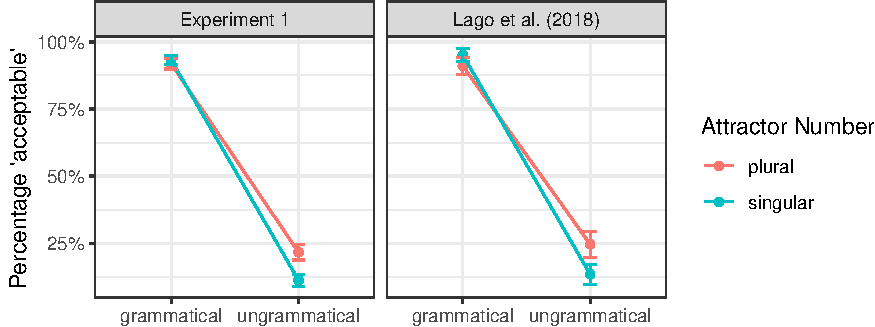
\includegraphics{paper_draft_files/figure-latex/exp1AvgResponse-1.pdf}
\caption{\label{fig:exp1AvgResponse}Estimates and 95\% credible intervals for the analysis of the probability of a \enquote{yes} response.}
\end{figure}

Figure \ref{fig:exp1AvgResponse} shows the percentages of \enquote{acceptable} answers for experiment 1 as well as the Lago et al.~data as a function of sentence grammaticality and the grammatical of number the attractor noun phrase. In our data, while ungrammatical sentences with a plural attractor were found acceptable in \% of the cases, the accepability rate was only \% when the attractor was singular.
This observed agreement attraction effect of \%, as well as the condition averages were fairly close to Lago et al.'s attraction effect of \%.

Figure \ref{fig:exp1ResponseModelPlot} shows the estimates of the fixed effects of a Bayesian hierarchical model. It shows that ungrammatical sentences were judged as acceptable far less often than grammatical sentences (CI = {[}XXX{]}). It also shows that sentences with plural attractors were considered acceptable a little bit better than sentences (CI = {[}XXX{]}) with singular attractors. Importantly, we found an interaction between these two factors, such that plural attractors increased the likelihood of \enquote{acceptable} responses disproportionately more in ungrammatical sentences (CI = {[}XXX{]}).

We found a small positive effect \ldots
evidence that the ambiguity of the head noun affects the effect of attractor number on ungrammaticality (CI = {[}XXX{]}).
\ldots no interesting difference between experiments \ldots
\ldots we may even have produced a bayes factor or LOO metric, to test whether that three way interaction actually matters
I see that the vowel ending is not significant even though it has a negative effect.
Thus, I may say that differentiating between the accusative case and the possessive suffix has caused a reduction in the effect of the agreement attraction. The results also show that when the attractor is plural, people have a high tendency to find the sentence grammatical.

\begin{verbatim}
## Warning: `expand_scale()` is deprecated; use `expansion()` instead.

## Warning: `expand_scale()` is deprecated; use `expansion()` instead.
\end{verbatim}

\begin{figure}
\centering
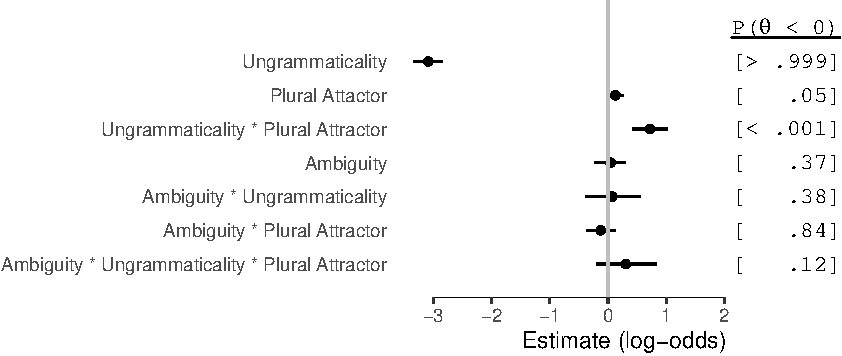
\includegraphics{paper_draft_files/figure-latex/exp1ResponseModelPlot-1.pdf}
\caption{\label{fig:exp1ResponseModelPlot}Estimates and 95\% credible intervals for the regression coefficients in accuracy (log-odds units).}
\end{figure}

\hypertarget{discussion}{%
\subsubsection{Discussion}\label{discussion}}

We replicated the number agreement attraction effect found by Lago et al. (2018), albeit with a larger sample size and while controlling for potential confound of head noun ambiguity. This finding suggests that the agreement attraction in Turkish is largely unaffected by the ambiguity of case marking of the head noun.
\ldots The small difference between the two experiments that we do find is quite likely due to the shorter response deadline in the Lago et al.~experiment. As a result of this short deadline, what we found in RT, they found in responses - i.e., in a slightly bigger agreement attraction effect
\ldots this finding has some relationship to the findings in Avetisyan et al. (n.d.)
\ldots however, Avetisyan et al. (n.d.)'s findings as such have more predictions -- for example, they predict that Lago et al.'s speculation about the role of genitive case in this attraction effect is likely wrong.

\ldots discuss the effect in fillers: the most likely explanation for this finding is that we messed up the fillers by not checking their accuracy. \ldots discuss
\ldots an alternative explanation is that we our fillers were ok, but the experiment design heavily biased participants towards \enquote{no} answers \ldots this appears unlikely since we got pretty much the same numbers as Lago et al., who didn't have such fillers (as far as I am aware) \ldots however, in case that is what happened, this does not change the interpretation of our finding, because \ldots

\hypertarget{section}{%
\subsection{}\label{section}}

Now that we replicated Lago et al.'s findings, it seems like all is good -- there is a number attraction effect in Turkish.

In my second experiment, I investigate the predictions made from my model using a verbal plural morpheme within a distractor relative clause. As mentioned earlier, the verbal plural morpheme in Turkish is exactly the same as the nominal plural with regards to its stress, its behavior, and its form: \emph{-lAr}. Since Turkish relative clauses are essentially nominals due to the nominalization process, they behave exactly like other nominals within the sentence (Erguvanlı-Taylan, 2015; Göksel \& Kerslake, 2004). They can be marked with cases, plural agreement and they can have postpositions that any nominal also can. This syntactic formation enables us to question how shallow people process, how much syntactic information is relevant, or how perfectly people encode the features of the elements of the sentence. In my experiment 2, I have used items in which the referential head noun of the subject is modified with a single-word relative clause as in \autoref{ouritem1}.

\begin{exe}
  \ex \label{ouritem1}
      \gll Döv-dük-(\textbf{ler})-i çocuk mutfak-ta baygın hal-de yat-ıyor-(\textbf{lar})-dı.\\
  beat-\textsc{Nmlz}-(\textsc{Pl})-\textsc{Poss} kid kitchen-\textsc{Loc} unconscious state-\textsc{Loc} lie-\textsc{Prog}-(\textsc{Pl})-\textsc{Pst}\\
      \glt Intended: The kid that they beat were laying in the kitchen unconscious.
\end{exe}

Within the framework of percolation theories, I expect a harsh decline in the agreement attraction effects\footnote{Discussion with regards to how and where relative clauses adjoined is omitted due to the scope of the paper. However, it should be clear that a late insertion analysis where the relative clauses are actually above the head noun would yield different results. In this paper, I assume that modifiers like relative clauses are within the noun phrase, which deems them \textit{syntactically} deeper placed in the hierarchical three than the possessee.}. The reason for this expected decline is the fact that relative clauses being relative \emph{deeper} in the hierarchical structure than the possessee of genitive-possessive structure.

As for cue-based retrieval models, I would expect an agreement attraction quite similar to the one that I originally have in Lago et al. (2018). The reason for this expected agreement attraction is the fact that apart from having a verbal root, the relative clauses and nominals behave exactly the same in terms of \emph{nounness}. Like nominals, nominalized structures first marked with plural and then with the case or possessive suffix. From this perspective, it seems like there should be no difference. However, one may argue that the features related to the verbal and nominal can be encoded differently. Thus, there will no partial match at any time given due to the fact that verbal plural morpheme at the main verb does specify cues for a specific type of plural marking. One other question that may arise from this structure is that whether or not the parts of already-formed dependencies can feed the following dependency resolution. In other words, the verbal plural morpheme \emph{-lar} on \emph{dövdükleri} in \autoref{ouritem1} is already a trigger of a cue retrieval process. And, when it is merged with the nominal head \emph{çocuk}, there is a formed semantic meaning that is \enquote{a group of people has beaten a kid.} However, this \emph{suggestion} assumes that relative clauses are formed at the very moment. Moreover, I also need to assume that after forming a relative clause they are unreachable, meaning that they do not contribute to the processing of the sentence, anymore.

Lastly, in my extremely shallow processing model, I would expect a significant effect of agreement attraction. Due to one of the writers' inability to \emph{run the numbers} and \emph{form the mpt trees in time}, this part---unfortunately---does not go beyond than a verbal argumentation. The reason I expect a significant effect of the agreement attraction is due to the fact that upon the agreement process is driven by the faulty memory of the place of the plural morpheme and uneducated guessing. Since the parsing is shallow, comprehenders do not engage in perfect attribution of the features, thus having a somewhat blurry representation behind. I expect this behavior to be omnipresent in other agreement attraction phenomenon that has been shown, as well as in Lago et al. (2018) and in my replication of it. Therefore, there is no reason to have anything to be different in experiment 2.

\begin{center}\rule{0.5\linewidth}{0.5pt}\end{center}

\hypertarget{experiment-2}{%
\subsection{Experiment 2}\label{experiment-2}}

Having discussed the replication study of Lago et al. (2018), I have shown that results favor the cue-based models, especially with the effect of disambiguated possessive suffix on response times. However, due to the extremely similar effects on agreement attraction, I can still entertain shallow processing mechanism as explained in \autoref{model1}, \autoref{model2}, and \autoref{model3}. Since I argue that the agreement attraction is a product of memory state in which comprehenders do not have an exact memory of the place of the plural morpheme mainly, I conducted an experiment where the distractor with the plural morpheme in on the relative clause.

The study consists of a speeded acceptability judgment experiment in the web-based platform Ibex Farm. In the experiment, I test whether or not speakers utilize even more shallow parser than what is stipulated by Lago et al. (2018) and my replication of Lago et al. (2018) Experiment 2. This was investigated using syntactic structures similar to Lago et al. (2018) materials, in which I have opted out the Genitive Construction (GC) for Relative Clause construction (RCC) as a distractor. In Turkish, like GC, the relative clause in RCC precedes the head noun, and length-wise Turkish relative clauses can consist of only one word and the rest can be dropped. Turkish allows us to use RCCs as distractors in the same place because Turkish plural morpheme in the verbal domain and nominal domain are the same: \emph{-lAr}. Both of them react similarly in the same phonological environments, and they also exhibit the same stress patterns.

In the experimental items, the distractor RC and the matrix verb had f my configurations in which the number morpheme on the RCC (\emph{plural} vs. \emph{singular} marked RC verb) and matrix verb (\emph{grammatical} vs. \emph{ungrammatical}) as in \autoref{prereg1}.

\begin{exe}
\ex \label{prereg1}
  \begin{xlist}
  \ex \textsc{Grammatical, SG attractor} \label{reg1}
      \gll Döv-düğ-ü çocuk okul-a yorgun arg?n gel-di.\\
  beat-\textsc{nmlz}-\textsc{poss} kid school-\textsc{dat} unconscious state-\textsc{loc} lie-\textsc{prog}-\textsc{pst}\\ 
      \glt The kid that he/she beats was laying in the kitchen unconscious.
  \ex \textsc{Grammatical, PL attractor} \label{reg2}
      \gll Döv-dük-ler-i çocuk mutfak-ta baygın hal-de yat-ıyor-du.\\
  beat-\textsc{nmlz}-\textsc{pl}-\textsc{poss} kid kitchen-\textsc{loc} unconscious state-\textsc{loc} lie-\textsc{prog}-\textsc{pst}\\
      \glt The kid that they beat was laying in the kitchen unconscious.
  \ex \textsc{Ungrammatical, PL attractor} \label{reg3}
      \gll Döv-dük-ler-i çocuk mutfak-ta baygın hal-de yat-ıyor-lar-dı.\\
  beat-\textsc{nmlz}-\textsc{pl}-\textsc{poss} kid kitchen-\textsc{loc} unconscious state-\textsc{loc} lie-\textsc{prog}-\textsc{pl}-\textsc{pst}\\
      \glt Intended: The kid that they beat were laying in the kitchen unconscious.
  \ex \textsc{Ungrammatical, SG attractor} \label{reg4}
      \gll Döv-düğ-ü çocuk mutfak-ta baygın hal-de yat-ıyor-lar-dı.\\
  beat-\textsc{nmlz}-\textsc{poss} kid kitchen-\textsc{loc} unconscious state-\textsc{loc} lie-\textsc{prog}-\textsc{pl}-\textsc{pst}\\
      \glt Intended: The kid that he/she beats were laying in the kitchen unconscious.
  \end{xlist}
\end{exe}

As for the experiment, I have used the same type of fillers with the Experiment 1 in order to tackle with two possible strategies that can be utilized by the participants: (i) deeming the sentence acceptable when the matrix verb is singular and (ii) deeming most of the sentences unacceptable when the matrix verb is plural. To tackle with the first type of strategy, I have used a sentence where the object is not marked with accusative and it is not in an immediately pre-verbal position as in \autoref{filler1a}. The idea was to have a singular matrix verb in an ungrammatical sentence where the ungrammaticality does not stem from the local elements. As for the other strategy I have used pro-drop characteristics of Turkish and made the first noun phrase with a relative clause an object as in \autoref{filler1b}. The idea behind is that the plural agreement on the matrix verb is resolved with a dropped subject instead of the first noun phrase with a relative clause. Every participant saw 40 experimental item that is Latin-squared and 40 fillers.

\begin{exe}
\ex
\begin{xlist}
\ex \label{filler1a}
\gll * Haberleş-tiğ-i çevirmen ara-ma-yınca metin keyfince bitir-di.\\
{\ } communicate-\textsc{Nmlz}-\textsc{Poss} translator call-\textsc{Neg}-\textsc{Nmlz} text as.he.wished finis-\textsc{Pst}\\
\glt Intended: ``When the translator that he spoke with did not call, he finished the text as he wished.''
\ex \label{filler1b}
\gll Sev-dik-ler-i öğretmen emekli ol-unca saatlerce ağla-dı-lar.\\
love-\textsc{Nmlz}-\textsc{Pl}-\textsc{Poss} teacher retired be-\textsc{Nmlz} for.hours cry-\textsc{Pst}-\textsc{Pl}\\
\glt ``When the teacher they loved retired, they cried for hours.''
\end{xlist}
\end{exe}

\hypertarget{participants-and-procedure-1}{%
\subsubsection{Participants and Procedure}\label{participants-and-procedure-1}}

Eighty Turkish speakers were recruited from Bogazici University in İstanbul. The procedure was exactly the same as Experiment 1. None of the participants in this experiment had participated in Experiment 1.

\hypertarget{analysis}{%
\subsubsection{Analysis}\label{analysis}}

Every experimental item from both experiments (this experiment and Experiment (1) is included in the analysis.
Participants for whom the difference between grammatical and ungrammatical sentences with no potential for agreement attraction (conditions c and d) did not exceed a threshold of \(0.25\) were deemed not to have performed the task as instructed, and their data was excluded from further analysis. In consequence, 1 participants' data was excluded.

Across participants, 31 trials were not responded to before the deadline (by 25 participants). The data from these trials was not used in the analysis of responses or reaction times.

We used \texttt{R} ({\textbf{???}}) and the \emph{tidyverse} R packages ({\textbf{???}}) for data processing and plotting, and the R packages \emph{brms} ({\textbf{???}} ``urkner\_2017; @B''urkner\_2018) and \emph{rstan} ({\textbf{???}}) to fit Bayesian hierarchical models (e.g., Gelman \& Hill, 2007; Gelman et al., 2014; McElreath, 2016).

Participants' responses were analyzed using Bayesian hierarchical generalized linear models using a Bernoulli distribution with a probit link. Models of response times were fit using the lognormal distribution. Both models were fit with the predictors
\ldots predictors \ldots

\hypertarget{results-1}{%
\subsubsection{Results}\label{results-1}}

\begin{figure}
\centering
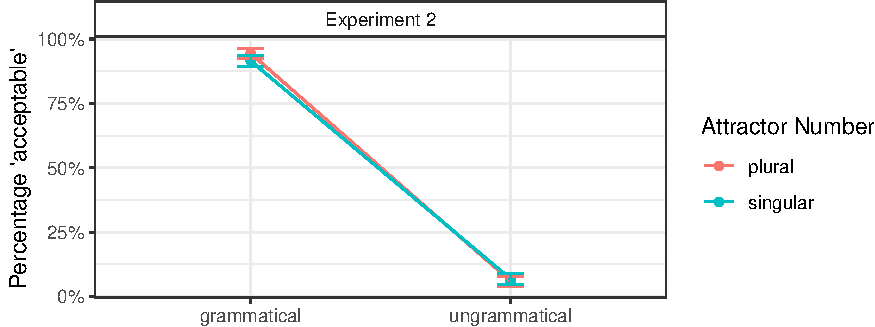
\includegraphics{paper_draft_files/figure-latex/exp2AvgResponse-1.pdf}
\caption{\label{fig:exp2AvgResponse}Estimates and 95\% credible intervals for the analysis of the probability of a \enquote{yes} response.}
\end{figure}

It is clear from Figure \ref{fig:exp2AvgResponse} that in the condition (c) where I expect an agreement attraction, participants find as unacceptable as the condition (d) with singular attractor, singular head noun, and plural matrix verb. While I do not see any agreement attraction (NA\%), I also see a more firm analysis of the ungrammatical sentence with singular matrix verb ((NA\%)).

As for the estimates of coefficients in \ref{fig:exp2ResponseModelPlot}, I can conclude that there is a significant negative effect of plural morpheme on the relative clause, which means that it does not cause any agreement affects. Again, the effect of ungrammaticality that stems from the existence of plural morpheme on the matrix verb is visible. The interaction between the plural morpheme on the attractor RC and the matrix verb is even higher than the sole effect of plural morpheme on the attractor RC.

\begin{figure}
\centering
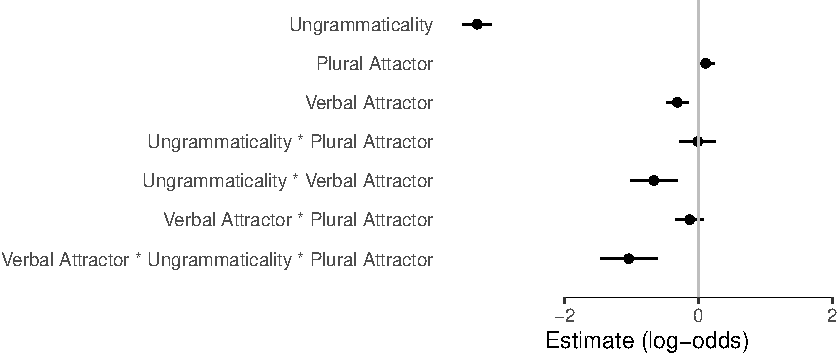
\includegraphics{paper_draft_files/figure-latex/exp2ResponseModelPlot-1.pdf}
\caption{\label{fig:exp2ResponseModelPlot}log-odd Estimates and 95\% credible intervals for the regression coefficients.}
\end{figure}

Finally, the response times of Experiment 2 is significantly lower than the Experiment 1 as seen from Figure FIX The even lower response time in ungrammatical plural (condition c) shows that participants were extremely confident with their decision and did not have any issue with the dependency resolution.

\hypertarget{discussion-1}{%
\subsubsection{Discussion}\label{discussion-1}}

These findings indicate that my hypothesis regarding the matching of the forms is not supported by the empirical evidence. However, results in Experiment 2 points in a direction where the Marking and Morphing studies predicted in the first place. Due to the deeper syntactic embedding, the numeral feature cannot percolate as freely as it can in genitive possessive structure and cannot affect the final number of the subject root node.

However, with the right prediction with regards to which features are stored and can be cued for, cue-based retrieval mechanisms can also explain the findings in Experiment 2.

\hypertarget{conclusion}{%
\section{Conclusion}\label{conclusion}}

We have shown that the agreement attraction effects cannot be explained by the extremely shallow processing mechanisms, at least with the implementation I have proposed here. However, I also show that findings from Experiment 1 and 2 were not enough to differentiate between two models that can explain agreement attraction: the Marking and Morphing and cue-based retrieval models. While the findings of Experiment 1 favors the cue-based retrieval mechanism, Experiment 2 with the harsh decline in the effects of agreement attraction points to another horizon.

Another take on the results may follow from the redefinition of the \emph{shallowness} concept. Experiments show that it is not only dependent on the form. However, it can be an issue related to already-formed dependencies inability to be used in the memory process. One can argue that once the dependencies are formed and resolved, participants do not go back to them when another cue is set out.

\hypertarget{references}{%
\section*{References}\label{references}}
\addcontentsline{toc}{section}{References}

\hypertarget{refs}{}
\leavevmode\hypertarget{ref-AvetisyanEtAl:2019}{}%
Avetisyan, S., Lago, S., \& Vasishth, S. (n.d.). Does case marking affect agreement attraction in comprehension? \url{https://doi.org/10.31234/OSF.IO/KMBGY}

\leavevmode\hypertarget{ref-BadeckerKuminiak:2007}{}%
Badecker, W., \& Kuminiak, F. (2007). Morphology, agreement and working memory retrieval in sentence production: Evidence from gender and case in Slovak. \emph{Journal of Memory and Language}, \emph{56}(1), 65--85.

\leavevmode\hypertarget{ref-Bock2001}{}%
Bock, K., Eberhard, K. M., Cutting, J. C., Meyer, A. S., \& Schriefers, H. (2001). Some attractions of verb agreement. \emph{Cognitive Psychology}, \emph{43}(2), 83--128.

\leavevmode\hypertarget{ref-Bock1991}{}%
Bock, K., \& Miller, C. A. (1991). Broken agreement. \emph{Cognitive Psychology}, \emph{23}(1), 45--93.

\leavevmode\hypertarget{ref-Dell1986}{}%
Dell, G. S. (1986). A spreading-activation theory of retrieval in sentence production. \emph{Psychological Review}, \emph{93}(3), 283.

\leavevmode\hypertarget{ref-Dillon2013}{}%
Dillon, B., Mishler, A., Sloggett, S., \& Phillips, C. (2013). Contrasting intrusion profiles for agreement and anaphora: Experimental and modeling evidence. \emph{Journal of Memory and Language}, \emph{69}(2), 85--103.

\leavevmode\hypertarget{ref-Eberhard2005}{}%
Eberhard, K. M., Cutting, J. C., \& Bock, K. (2005). Making syntax of sense: Number agreement in sentence production. \emph{Psychological Review}, \emph{112}(3), 531.

\leavevmode\hypertarget{ref-EnochsonCulbertson:2015}{}%
Enochson, K., \& Culbertson, J. (2015). Collecting psycholinguistic response time data using Amazon Mechanical Turk. \emph{PLoS ONE}, \emph{10}(3), 1--17. \url{https://doi.org/10.1371/journal.pone.0116946}

\leavevmode\hypertarget{ref-Taylan2015}{}%
Erguvanlı-Taylan, E. (2015). \emph{The phonology and morphology of turkish}. Boğaziçi Üniversitesi.

\leavevmode\hypertarget{ref-Franck2006}{}%
Franck, J., Lassi, G., Frauenfelder, U. H., \& Rizzi, L. (2006). Agreement and movement: A syntactic analysis of attraction. \emph{Cognition}, \emph{101}(1), 173--216.

\leavevmode\hypertarget{ref-Franck2015}{}%
Franck, J., \& Wagers, M. W. (2015). Hierarchical structure and memory retrieval mechanisms in attraction: An sat study. In \emph{28th annual cuny conference on human sentence processing}.

\leavevmode\hypertarget{ref-BDA3}{}%
Gelman, A., Carlin, J. B., Stern, H. S., Dunson, D. B., Vehtari, A., \& Rubin, D. B. (2014). \emph{Bayesian Data Analysis} (3rd ed.). London: CRC/Chapman-Hall.

\leavevmode\hypertarget{ref-GelmanHill:2007}{}%
Gelman, A., \& Hill, J. (2007). \emph{Data Analysis Using Regression and Multilevel/Hierarchical Models}. Cambridge, UK: Cambridge University Press.

\leavevmode\hypertarget{ref-Goksel2004}{}%
Göksel, A., \& Kerslake, C. (2004). \emph{Turkish: A comprehensive grammar}. Routledge.

\leavevmode\hypertarget{ref-HammerlyEtAl:2019}{}%
Hammerly, C., Staub, A., \& Dillon, B. (2019). The grammaticality asymmetry in agreement attraction reflects response bias: Experimental and modeling evidence. \emph{Cognitive Psychology}, \emph{110}(January), 70--104. \url{https://doi.org/10.1016/j.cogpsych.2019.01.001}

\leavevmode\hypertarget{ref-Hartsuiker2001}{}%
Hartsuiker, R. J., Antón-Méndez, I., \& Van Zee, M. (2001). Object attraction in subject-verb agreement construction. \emph{Journal of Memory and Language}, \emph{45}(4), 546--572.

\leavevmode\hypertarget{ref-Kimball1971}{}%
Kimball, J., \& Aissen, J. (1971). I think, you think, he think. \emph{Linguistic Inquiry}, \emph{2}(2), 241--246.

\leavevmode\hypertarget{ref-KwonSturt:2016}{}%
Kwon, N., \& Sturt, P. (2016). Attraction Effects in Honorific Agreement in Korean. \emph{Frontiers in Psychology}, \emph{7}(August), 1--13. \url{https://doi.org/10.3389/fpsyg.2016.01302}

\leavevmode\hypertarget{ref-LagoEtAl:2018}{}%
Lago, S., Felser, C., Gračanin-Yuksek, M., Demir, O., Kırkıcı, B., \& Şafak, D. F. (2018). Straight from the horse's mouth: Agreement attraction effects with Turkish possessors. \emph{Linguistic Approaches to Bilingualism}, \emph{12}(1), 1--29. \url{https://doi.org/10.1075/lab.17019.lag}

\leavevmode\hypertarget{ref-LagoEtAl:2015}{}%
Lago, S., Shalom, D. E., Sigman, M., Lau, E. F., \& Phillips, C. (2015). Agreement attraction in Spanish comprehension. \emph{Journal of Memory and Language}, \emph{82}, 133--149. \url{https://doi.org/10.1016/j.jml.2015.02.002}

\leavevmode\hypertarget{ref-Lewis2005}{}%
Lewis, R. L., \& Vasishth, S. (2005). An activation-based model of sentence processing as skilled memory retrieval. \emph{Cognitive Science}, \emph{29}(3), 375--419.

\leavevmode\hypertarget{ref-Lewis2006}{}%
Lewis, R. L., Vasishth, S., \& Van Dyke, J. A. (2006). Computational principles of working memory in sentence comprehension. \emph{Trends in Cognitive Sciences}, \emph{10}(10), 447--454.

\leavevmode\hypertarget{ref-McElreath:2016}{}%
McElreath, R. (2016). \emph{Statistical rethinking: A bayesian course with examples in R and Stan.} Boca Raton: CRC Press.

\leavevmode\hypertarget{ref-NicolEtAl:2016}{}%
Nicol, J. L., Barss, A., \& Barker, J. E. (2016). Minimal interference from possessor phrases in the production of subject-verb agreement. \emph{Frontiers in Psychology}, \emph{7}(MAY), 1--12. \url{https://doi.org/10.3389/fpsyg.2016.00548}

\leavevmode\hypertarget{ref-PatsonHusband:2015}{}%
Patson, N. D., \& Husband, E. M. (2015). Misinterpretations in agreement and agreement attraction. \emph{Quarterly Journal of Experimental Psychology}, \emph{0218}(February), 1--22. \url{https://doi.org/10.1080/17470218.2014.992445}

\leavevmode\hypertarget{ref-ReifegersteEtAl:2016}{}%
Reifegerste, J., Hauer, F., \& Felser, C. (2016). Agreement processing and attraction errors in aging: evidence from subject-verb agreement in German. \emph{Aging, Neuropsychology, and Cognition}, \emph{00}(00), 1--31. \url{https://doi.org/10.1080/13825585.2016.1251550}

\leavevmode\hypertarget{ref-SlioussarMalko:2016}{}%
Slioussar, N., \& Malko, A. (2016). Gender agreement attraction in Russian: production and comprehension evidence, \emph{7}(November), 1--20. \url{https://doi.org/10.3389/fpsyg.2016.01651}

\leavevmode\hypertarget{ref-TannerEtAl:2014}{}%
Tanner, D., Nicol, J., \& Brehm, L. (2014). The time-course of feature interference in agreement comprehension: Multiple mechanisms and asymmetrical attraction. \emph{Journal of Memory and Language}, \emph{76}, 195--215. \url{https://doi.org/10.1016/j.jml.2014.07.003}

\leavevmode\hypertarget{ref-TuckerEtAl:2015}{}%
Tucker, M. A., Idrissi, A., \& Almeida, D. (2015). Representing number in the real-time processing of agreement: Self-paced reading evidence from Arabic. \emph{Frontiers in Psychology}, \emph{6}(MAR), 1--21. \url{https://doi.org/10.3389/fpsyg.2015.00347}

\leavevmode\hypertarget{ref-WagersEtAl:2009}{}%
Wagers, M. W., Lau, E. F., \& Phillips, C. (2009). Agreement attraction in comprehension: Representations and processes. \emph{Journal of Memory and Language}, \emph{61}(2), 206--237. \url{https://doi.org/10.1016/j.jml.2009.04.002}

\end{document}
